
The analysis presented takes an inclusive approach to its background estimation strategies. 
Instead of separating backgrounds based on the number of fake taus or origin of fake taus,  the backgrounds are estimated based on the underlying \ac{SM} process,  including prompt and fake tau leptons. 
\ac{SM} processes dominated by QCD interactions, leading to multiple jets in the final state, can enter a di-tau final state through at least one jet being misidentified as hadronically decaying tau lepton. This background is estimated via a so called "ABCD" method. $W$+ jets events can similarly end up in a di-tau final state through at least one fake tau. A muon plus tau final state is used to normalise the Monte Carlo estimation of this process.
Since top related backgrounds (with and without fake taus) are the leading contribution to the high mass signal region, an additional estimation of this background in a control region is performed.
To validate the modelling of WW and WZ processes contributing to the SR-C1N2SS-HM, a validation region was designed, using a pair of opposite-sign muons to enhance the statistics of this process.
%====================================================================================================
%==============================================Multijet estimation ==================================
%====================================================================================================

\subsection{Estimation of Multi-jet background}
\label{sec:bkgestimation:ABCD}

The multi-jet \ac{SM} background includes all strong interactions producing a final state with multiple jets.  Due to the similarity of jets and tau signatures,  this process is populating the final state considered in this analysis of at least two hadronically decaying taus.  In contrast to the \ac{SUSY} signal model of interest,  this standard model process does not have large \Met. Any missing transverse energy in the events is caused by mismeasurements.  A quark or gluon jet could be misidentified as a one or three-prong tau,  discarding some of the \ac{ID} tracks that would otherwise be taken into account in the jet momentum.  These unaccounted tracks can increase the instrumental \Met. 
Due to the instrumental origin of the \Met in the event,  the multi-jet processes predominantly populate phase space regions with low missing transverse momenta.  
Since the multijet background originates in soft QCD processes,  its simulation through Monte Carlo generators is unreliable,  especially in high momentum phase spaces considered in this analysis. 
A data-driven estimation method,  the \textit{ABCD} method, is therefore used to extract a multi-jet estimation from data. 

Two kinematic variables are used to construct a set of orthogonal regions: the tau identification working point of the leading two taus and sum of the \Mt of the two leading taus.
%and  is used to increase the population of multi-jet events.  As discussed in section \ref{sec:DAQ:ObjectReco:Taus},  the tau identification working point is using a \ac{RNN} to distinguish between jets and hadronically decaying taus. Therefore, lowering the tau ID working point increases the amount of non-prompt taus.
%fis the second parameter,  spanning up a space that allows targeting similar events as in the signal regions or looser restrictions. 
Any additional cuts that have been defined in the signal region optimisation are not applied to the control and validation regions built for the ABCD method. 
A sketch of the regions described is given in figure \ref{fig:bkgestimation:QCD:sketch}.
A detailed definition of the kinematic cuts applied to the regions in order to define the ABCD regions is given in table \ref{tab:bkgestimation:QCD:table}. The signal region phase spaces present the regions denoted as D within this methodology. \\

\begin{figure}[h]
  \subfloat[Low mass ABCD regions]{
		\centering
	\scalebox{0.9}{
		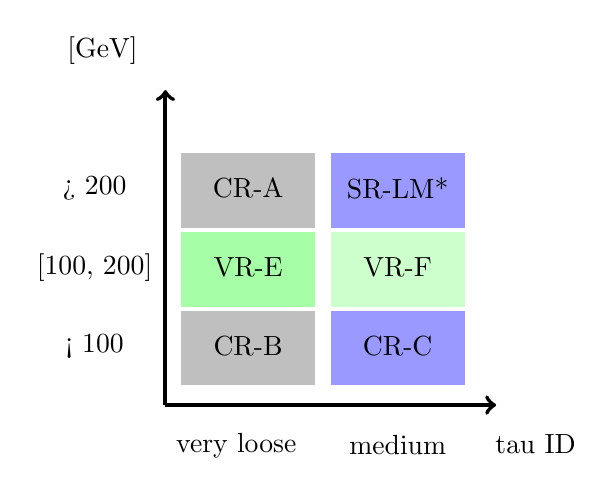
\begin{tikzpicture}
		\draw[line width =1.5pt,->] (0,0) -- (4.2,0);
		\node[](A) at (4.7,-0.5) {tau ID};
		\draw[line width =1.5pt,->] (0,0) -- (0,4.0);
		\node[](B) at (-0.8,4.5) {\Summt [GeV]};
		\node[](D) at (0.9, -0.51) {very loose };
		\node[](D) at (2.95, -0.50) {medium };
		\fill[gray!50] (0.2,0.25) rectangle (1.9,1.2);
		\node[](E) at (1.05,0.75) {CR-B};
		\node[](F)  at (-0.9,0.75) {< 100};
		\fill[green!35] (0.2,1.25) rectangle (1.9,2.2);
		\node[](G) at (1.05,1.75) {VR-E};
		\node[](H)  at (-0.9,1.75) {[100, 200]};
		\fill[gray!50] (0.2,2.25) rectangle (1.9,3.2);
		\node[](I) at (1.05,2.75) {CR-A};
		\node[](J)  at (-0.9,2.75) {> 200};
		\fill[blue!40] (2.1,0.25) rectangle (3.8,1.2);
		\node[](K) at (2.95,0.75) {CR-C};
		\fill[green!20] (2.1,1.25) rectangle (3.8,2.2);
		\node[](L) at (2.95,1.75) {VR-F};
		\fill[blue!40] (2.1,2.25) rectangle (3.8,3.2);
		\node[](M) at (2.95,2.75) {SR-LM*};
		\end{tikzpicture} }}
		  \subfloat[High mass ABCD regions]{
		\centering
	\scalebox{0.9}{
		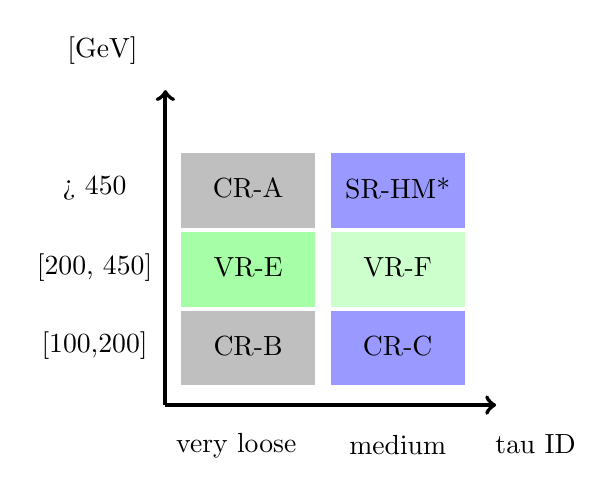
\begin{tikzpicture}
		\draw[line width =1.5pt,->] (0,0) -- (4.2,0);
		\node[](A) at (4.7,-0.5) {tau ID};
		\draw[line width =1.5pt,->] (0,0) -- (0,4.0);
		\node[](B) at (-0.8,4.5) {\Summt [GeV]};
		\node[](D) at (0.9, -0.51) {very loose };
		\node[](D) at (2.95, -0.50) {medium };
		\fill[gray!50] (0.2,0.25) rectangle (1.9,1.2);
		\node[](E) at (1.05,0.75) {CR-B};
		\node[](F)  at (-0.9,0.75) {[100,200]};
		\fill[green!35] (0.2,1.25) rectangle (1.9,2.2);
		\node[](G) at (1.05,1.75) {VR-E};
		\node[](H)  at (-0.9,1.75) {[200, 450]};
		\fill[gray!50] (0.2,2.25) rectangle (1.9,3.2);
		\node[](I) at (1.05,2.75) {CR-A};
		\node[](J)  at (-0.9,2.75) {> 450};
		\fill[blue!40] (2.1,0.25) rectangle (3.8,1.2);
		\node[](K) at (2.95,0.75) {CR-C};
		\fill[green!20] (2.1,1.25) rectangle (3.8,2.2);
		\node[](L) at (2.95,1.75) {VR-F};
		\fill[blue!40] (2.1,2.25) rectangle (3.8,3.2);
		\node[](M) at (2.95,2.75) {SR-HM*};
		\end{tikzpicture}}
}
\caption{ABCD region illustration for the low and high mass signal regions \label{fig:bkgestimation:QCD:sketch} Here only the cuts on \Summt and the tau-ID are shown.  $^*$ As described in section \ref{sec:analysis:sroptimisation},  further requirements on other kinematic variables are applied to define the signal regions}
\end{figure}

\begin{table}[ht!]
\centering
\footnotesize
\begin{tabular}{|c|c||c|c|}
\hline 
\textbf{CR-A} & \textbf{SR-LM} & \textbf{CR-A} & \textbf{SR-HM}\tabularnewline
\hline 
\hline 
$\geq$2 very loose or loose $\tau$'s & $\geq$2 medium $\tau$'s & $\geq$2 very loose or loose $\tau$'s & $\geq$2 medium $\tau$'s\tabularnewline
\textless{} 2 medium $\tau$'s & - & \textless{} 2 medium $\tau$'s & -\tabularnewline
$m_{Tsum}\geq200$ GeV & $m_{Tsum}\geq200$ GeV & $m_{Tsum}\geq450$ GeV & $m_{Tsum}\geq450$ GeV\tabularnewline
$\Delta\Phi(\tau_{1},\tau_{2})\geq1.5$ & $\Delta\Phi(\tau_{1},\tau_{2})\geq1.5$ & \Met $\geq$50 GeV & \Met $\geq$150 GeV\tabularnewline
\hline 
\hline 
\textbf{VR-E} & \textbf{VR-F} & \textbf{VR-E} & \textbf{VR-F}\tabularnewline
\hline 
\hline 
$\geq$2 very loose or loose $\tau$'s & $\geq$2 medium $\tau$'s & $\geq$2 very loose or loose $\tau$'s & $\geq$2 medium $\tau$'s\tabularnewline
\textless{} 2 medium $\tau$'s & - & \textless{} 2 medium $\tau$'s & -\tabularnewline
$m_{Tsum}$ $\in$ $[100,200]$ GeV & $m_{Tsum}$ $\in$ $[100,200]$ GeV & $m_{Tsum}$ $\in$ $[200,450]$ GeV & $m_{Tsum}$ $\in$ $[200,450]$ GeV\tabularnewline
$\Delta\Phi(\tau_{1},\tau_{2})\leq1.5$ & $\Delta\Phi(\tau_{1},\tau_{2})\leq1.5$ & \Met $\geq$50 GeV & \Met $\geq$50 GeV\tabularnewline
\hline 
\hline 
\textbf{CR-B} & \textbf{CR-C} & \textbf{CR-B} & \textbf{CR-C}\tabularnewline
\hline 
\hline 
$\geq$2 very loose or loose $\tau$'s & $\geq$2 medium $\tau$'s & $\geq$2 very loose or loose $\tau$'s & $\geq$2 medium $\tau$'s\tabularnewline
\textless{} 2 medium $\tau$'s & - & \textless{} 2 medium $\tau$'s & -\tabularnewline
$m_{Tsum}<100$ GeV & $m_{Tsum}<100$ GeV & $m_{Tsum}$ $\in$ $[100,200]$ GeV & $m_{Tsum}$ $\in$ $[100,200]$ GeV\tabularnewline
$\Delta\Phi(\tau_{1},\tau_{2})\leq1.5$ & $\Delta\Phi(\tau_{1},\tau_{2})\leq1.5$ & \Met $\geq$50 GeV & \Met $\geq$50 GeV\tabularnewline
\hline 
\end{tabular}
\caption{The multi-jet control region and validation region
  definitions for signal regions described in Table~\ref{tab:SRdef}.
  Only those requirements regarding the \Summt that are different in the CRs/VRs with
  respect to the SRs are listed. \label{tab:bkgestimation:QCD:table}}
\end{table}

%
%\begin{table}[ht!]
%\centering
%\footnotesize
%\smallskip
%\begin{tabular}{c|c}
%\toprule
%% AD------------------
%$\mathbf {CR-A~}$ & $\mathbf {SR-LM}$\\
%\hline
%$\ge$ 2 very loose or loose $\tau$s       & $\ge$ 2 medium $\tau$s (SS)   \\
%$<$ 2 medium $\tau$s     &      --      \\
%$m_{Tsum}\geq 200 \text{ GeV} $ &  $m_{Tsum}\geq 200 \text{ GeV} $      \\ %SumMtCut
%$\Delta \Phi(\tau_1,\tau_2) \geq 1.5 $ &  $\Delta \Phi(\tau_1,\tau_2) \geq 1.5 $ \\ %DeltaPhiCut
%\hline
%%EF---------------
%\hline
%$\mathbf {VR-E~}$ & $\mathbf {VR-F~}$ \\
%\hline                                                      \hline
%$\ge$ 2 very loose or loose $\tau$s       & $\ge$ 2 medium $\tau$s (SS)   \\
%$<$ 2 medium $\tau$s     &      --      \\
%$m_{Tsum}\in [100,200] \text{ GeV} $ &  $m_{Tsum}\in [100,200] \text{ GeV} $      \\ %SumMtCut
%$\Delta \Phi(\tau_1,\tau_2) \leq 1.5 $ &  $\Delta \Phi(\tau_1,\tau_2) \leq 1.5 $ \\ %DeltaPhiCut
%\hline
%% BC-----------------
%\hline
%$\mathbf {CR-B~}$ & $\mathbf {CR-C~}$ \\
%\hline                                                      \hline
%$\ge$ 2 very loose or loose $\tau$s       &  $\ge$ 2 medium $\tau$s (SS)   \\
%$<$ 2 medium $\tau$s     &      --      \\
%$m_{Tsum}< 100 \text{ GeV} $ &  $m_{Tsum}< 100 \text{ GeV} $      \\ %SumMtCut
%$\Delta \Phi(\tau_1,\tau_2) \leq 1.5 $ &  $\Delta \Phi(\tau_1,\tau_2) \leq 1.5 $ \\ %DeltaPhiCut
%\hline
%\bottomrule
%\end{tabular}
%\smallskip
%\begin{tabular}{c|c}
%\toprule
%% AD------------------
%$\mathbf {CR-A~}$ & $\mathbf {SR-HM}$\\
%\hline
%$\ge$ 2 very loose or loose $\tau$s       & $\ge$ 2 medium $\tau$s (SS)   \\
%$<$ 2 medium $\tau$s     &      --      \\
%$m_{Tsum}\geq 450 \text{ GeV} $ &  $m_{Tsum}\geq 450 \text{ GeV} $      \\ %SumMtCut
%$E_T^\text{miss} \geq 50 \text{ GeV} $ & $E_T^\text{miss} \geq 150 \text{ GeV} $ \\ %met cut
%\hline
%%EF---------------
%\hline
%$\mathbf {VR-E~}$ & $\mathbf {VR-F~}$\\
%\hline                                                      \hline
%$\ge$ 2 very loose or loose $\tau$s       & $\ge$ 2 medium $\tau$s (SS)   \\
%$<$ 2 medium $\tau$s     &      --      \\
%$m_{Tsum}\in [200,450] \text{ GeV} $ &  $m_{Tsum}\in [200,450] \text{ GeV} $      \\ %SumMtCut
%$E_T^\text{miss} \geq 50 \text{ GeV} $ & $E_T^\text{miss} \geq 50 \text{ GeV} $ \\ %met cut
%\hline
%% BC-----------------
%\hline
%$\mathbf {CR-B~}$ & $\mathbf {CR-C~}$ \\
%\hline                                                      \hline
%$\ge$ 2 very loose or loose $\tau$s       &  $\ge$ 2 medium $\tau$s (SS)   \\
%$<$ 2 medium $\tau$s     &      --      \\
%$m_{Tsum} \in [100,200] \text{ GeV} $ &  $m_{Tsum} \in [100,200] \text{ GeV} $      \\ %SumMtCut
%$E_T^\text{miss} \geq 50 \text{ GeV} $ & $E_T^\text{miss} \geq 50 \text{ GeV} $ \\ %met cut
%\hline
%\bottomrule
%\end{tabular}
%\caption{The multi-jet control region and validation region
%  definitions for signal regions described in Table~\ref{tab:SRdef}.
%  Only those requirements regarding the \Summt that are different in the CRs/VRs with
%  respect to the SRs are listed. \label{tab:bkgestimation:QCD:table}}
%\end{table}

The multi-jet (MJ) contribution in CR-B and CR-C is obtained from the data yields in the respective regions,  with all other background contributions from Monte Carlo simulation subtracted;

\begin{align}
N^{MJ}_{CR-B/C} =  N^{data}_{CR-B/C} - N^{MC}_{CR-B/C} 
\end{align}

a transfer factor is extracted from the yields in CR-B and CR-C to extrapolate the multi-jet contribution to the medium ID validation and signal regions (VR-F and SR). 

\begin{align}
TF = \frac{N^{MJ}_{CR-C}}{N^{MJ}_{CR-B}}
\label{eq:bkgestimation:TF}
\end{align}

The systematic uncertainty on the transfer factor is estimated in the validation regions using formula \eqref{eq:bkgestimation:deltaTF} and is visualised in Figure \ref{fig:bkgestimation:ABCD:TF}.

\begin{align}
\Delta(TF)_{sys} =  | \frac{N^{MJ}_{CR-C}}{N^{MJ}_{CR-B}} - \frac{N^{MJ}_{VR-F}}{N^{MJ}_{VR-E}} | \label{eq:bkgestimation:deltaTF}
\end{align}

\begin{figure}[!htpb]
  \centering
%\subfloat[Low Mass]{\includegraphics[width=0.45\textwidth]{figures/C1N2SS/ABCD_closures/TF_SumMt_asymMT2False.pdf}}
\subfloat[Low Mass]{\includegraphics[width=0.45\textwidth]{figures/C1N2SS/ABCD_closures_noATLAS/TF_SumMtADT_asymMT2False.pdf}}
%\subfloat[High Mass]{\includegraphics[width=0.45\textwidth]{figures/C1N2SS/ABCD_closures/TF_SumMt_ditauMETMT2False.pdf}}
\subfloat[High Mass]{\includegraphics[width=0.45\textwidth]{figures/C1N2SS/ABCD_closures_noATLAS/TF_SumMtDTM_ditauMETMT2False.pdf}}
\caption{Dependency of the transfer factor on \Summt for low mass and high mass regions. Highlighted in the lower panel in red is the nominal used transfer factor value. All uncertainties are statistical only. \label{fig:bkgestimation:ABCD:TF}}
\end{figure}

%%----- result
The multi-jet yield in the signal region is then given by the multi-jet contribution in CR-A (given through data subtracted by other \ac{SM} contributions from Monte Carlo simulation) multiplied by the transfer factor with additional cuts.
The results of the ABCD method are summarised in Table
\ref{tab:bkgestimation:ABCDresults}. The SM predictions are in agreement with
the observed data counts in the multi-jet validation regions, as shown in Table \ref{tab:bkgestimation:VRFresults}.
%The systematic uncertainties of the ABCD method are discussed in
%Section \ref{sec:syst_ABCD}.

%\begin{table}
%\centering
%\tiny
%  \begin{tabular}{c|c|c|c|c|c|c|c|c}
%  \hline
%  & Sample & CR-B & CR-C & VR-E & CR-A & T=C/B & multi-jet in VR-F & multi-jet in SR-D\tabularnewline
%  \hline
%  \hline
%  \multirow{7}{*}{LM} & \textbf{Data} & \textbf{585} & \textbf{65} & \textbf{356} & \textbf{1505} & \multirow{2}{*}{} & \multirow{7}{*}{$19.55 \pm 1.13$} & \multirow{7}{*}{$0.94\pm0.27$}\tabularnewline
%%  \cline{2-2}
%   & $Z$+ jets & $11.70\pm2.11$ & $25.92\pm2.70$ & $3.62\pm1.06$ & $32.85\pm11.07$ &  &  & \tabularnewline
%  \cline{2-2}
%   & $W$+ jets & $4.84\pm2.35$ & $3.29\pm0.96$ & $11.48\pm4.67$ & $32.21\pm10.06$ & $0.058$ &  & \tabularnewline
%  \cline{2-2}
%   & Multiboson & $0.80\pm0.38$ & $2.04\pm0.35$ & $1.20\pm0.40$ & $2.18\pm0.50$ & $\pm0.015$ &  & \tabularnewline
%  \cline{2-2}
%   & Top & $2.54\pm0.75$ & $0.16\pm0.27$ & $2.45\pm0.88$ & $5.24\pm0.93$ & $\pm0.020$ &  & \tabularnewline
%  \cline{2-2}
%   & Higgs & $0.13\pm0.04$ & $0.73\pm0.09$ & $0.09\pm0.05$ & $0.53\pm0.46$ & \multirow{2}{*}{} &  & \tabularnewline
%  \cline{2-2}
%   & \emph{Multi-jet} & $564.98\pm24.41$ & $32.86\pm8.57$ & $337.16\pm19.49$ & $1431.98\pm41.59$ &  &  & \tabularnewline
%  \hline
%  \hline
%  \multirow{7}{*}{HM} & \textbf{Data} & \textbf{2185} & \textbf{309} & \textbf{3651} & \textbf{14} & \multirow{2}{*}{} & \multirow{7}{*}{$283.10 \pm 7.738$} & \multirow{7}{*}{$-0.086\pm0.31$}\tabularnewline
%  \cline{2-2}
%   & $Z$+ jets & $30.81\pm7.41$ & $32.53\pm10.81$ & $56.12\pm17.74$ & $2.64\pm1.37$ &  &  & \tabularnewline
%  \cline{2-2}
%   & $W$+ jets & $178.87\pm51.40$ & $74.13\pm15.33$ & $248.68\pm64.10$ & $6.35\pm2.58$ & $0.086$ &  & \tabularnewline
%  \cline{2-2}
%   & Multiboson & $6.03\pm0.87$ & $18.35\pm0.97$ & $14.42\pm1.44$ & $0.83\pm0.29$ & $\pm0.014$ &  & \tabularnewline
%  \cline{2-2}
%   & Top & $20.73\pm2.01$ & $14.38\pm1.53$ & $39.23\pm2.72$ & $2.10\pm0.57$ & $\pm0.011$ &  & \tabularnewline
%  \cline{2-2}
%   & Higgs & $0.53\pm0.38$ & $1.27\pm0.58$ & $0.71\pm0.47$ & $0.01\pm0.00$ & \multirow{2}{*}{} &  & \tabularnewline
%  \cline{2-2}
%   & \emph{Multi-jet} & $1948.04\pm69.90$ & $168.34\pm25.78$ & $3291.83\pm89.91$ & $2.07\pm4.79$ &  &  & \tabularnewline
%  \hline
%  \end{tabular}
%  \caption{Monte Carlo  backgrounds in the ABCD regions of the signal
%  regions defined in Table \ref{tab:SRdef}. The uncertainties given
%  on the transfer factor are both statistical and systematic
%  uncertainties. \label{tab:bkgestimation:ABCDresults} }
%\end{table}

\begin{table}
\centering {\tiny{}}%
\begin{tabular}{|c|c|c|c|c|c|c|c|c|}
\hline 
\multirow{2}{*}{} & \multirow{2}{*}{\textbf{\tiny{}Sample }} & \multirow{2}{*}{\textbf{\tiny{}CR-B }} & \multirow{2}{*}{\textbf{\tiny{}CR-C }} & \multirow{2}{*}{\textbf{\tiny{}VR-E }} & \multirow{2}{*}{\textbf{\tiny{}CR-A }} & \multirow{2}{*}{\textbf{\tiny{}T=C/B}{\tiny{} }} & \textbf{\tiny{}multi-jet } & \textbf{\tiny{}multi-jet }\tabularnewline
 &  &  &  &  &  &  & \textbf{\tiny{}in VR-F } & \textbf{\tiny{}in SR-C1N2SS}\tabularnewline
\hline 
\hline 
\multirow{7}{*}{\textbf{\tiny{}LM}} & \textbf{\tiny{}Data}{\tiny{} } & \textbf{\tiny{}585}{\tiny{} } & \textbf{\tiny{}65}{\tiny{} } & \textbf{\tiny{}356}{\tiny{} } & \textbf{\tiny{}1505}{\tiny{} } & \multirow{2}{*}{} & \multirow{7}{*}{{\tiny{}$19.55\pm1.13$}} & \multirow{7}{*}{{\tiny{}$0.94\pm0.27$}}\tabularnewline
\cline{2-6} \cline{3-6} \cline{4-6} \cline{5-6} \cline{6-6} 
 & {\tiny{}$Z$+ jets } & {\tiny{}$11.70\pm2.11$ } & {\tiny{}$25.92\pm2.70$ } & {\tiny{}$3.62\pm1.06$ } & {\tiny{}$32.85\pm11.07$ } &  &  & \tabularnewline
\cline{2-6} \cline{3-6} \cline{4-6} \cline{5-6} \cline{6-6} 
 & {\tiny{}$W$+ jets } & {\tiny{}$4.84\pm2.35$ } & {\tiny{}$3.29\pm0.96$ } & {\tiny{}$11.48\pm4.67$ } & {\tiny{}$32.21\pm10.06$ } & {\tiny{}$0.058$ } &  & \tabularnewline
\cline{2-6} \cline{3-6} \cline{4-6} \cline{5-6} \cline{6-6} 
 & {\tiny{}Multi-boson } & {\tiny{}$0.80\pm0.38$ } & {\tiny{}$2.04\pm0.35$ } & {\tiny{}$1.20\pm0.40$ } & {\tiny{}$2.18\pm0.50$ } & {\tiny{}$\pm0.015$ } &  & \tabularnewline
\cline{2-6} \cline{3-6} \cline{4-6} \cline{5-6} \cline{6-6} 
 & {\tiny{}Top } & {\tiny{}$2.54\pm0.75$ } & {\tiny{}$0.16\pm0.27$ } & {\tiny{}$2.45\pm0.88$ } & {\tiny{}$5.24\pm0.93$ } & {\tiny{}$\pm0.020$ } &  & \tabularnewline
\cline{2-6} \cline{3-6} \cline{4-6} \cline{5-6} \cline{6-6} 
 & {\tiny{}Higgs } & {\tiny{}$0.13\pm0.04$ } & {\tiny{}$0.73\pm0.09$ } & {\tiny{}$0.09\pm0.05$ } & {\tiny{}$0.53\pm0.46$ } & \multirow{2}{*}{} &  & \tabularnewline
\cline{2-6} \cline{3-6} \cline{4-6} \cline{5-6} \cline{6-6} 
 & \emph{\tiny{}Multi-jet}{\tiny{} } & {\tiny{}$564.98\pm24.41$ } & {\tiny{}$32.86\pm8.57$ } & {\tiny{}$337.16\pm19.49$ } & {\tiny{}$1431.98\pm41.59$ } &  &  & \tabularnewline
\hline 
\multirow{7}{*}{\textbf{\tiny{}HM}} & \textbf{\tiny{}Data}{\tiny{} } & \textbf{\tiny{}2185}{\tiny{} } & \textbf{\tiny{}309}{\tiny{} } & \textbf{\tiny{}3651}{\tiny{} } & \textbf{\tiny{}14}{\tiny{} } & \multirow{2}{*}{} & \multirow{7}{*}{{\tiny{}$283.10\pm7.738$}} & \multirow{7}{*}{{\tiny{}$-0.086\pm0.31$}}\tabularnewline
\cline{2-6} \cline{3-6} \cline{4-6} \cline{5-6} \cline{6-6} 
 & {\tiny{}$Z$+ jets } & {\tiny{}$30.81\pm7.41$ } & {\tiny{}$32.53\pm10.81$ } & {\tiny{}$56.12\pm17.74$ } & {\tiny{}$2.64\pm1.37$ } &  &  & \tabularnewline
\cline{2-6} \cline{3-6} \cline{4-6} \cline{5-6} \cline{6-6} 
 & {\tiny{}$W$+ jets } & {\tiny{}$178.87\pm51.40$ } & {\tiny{}$74.13\pm15.33$ } & {\tiny{}$248.68\pm64.10$ } & {\tiny{}$6.35\pm2.58$ } & {\tiny{}$0.086$ } &  & \tabularnewline
\cline{2-6} \cline{3-6} \cline{4-6} \cline{5-6} \cline{6-6} 
 & {\tiny{}Multi-boson } & {\tiny{}$6.03\pm0.87$ } & {\tiny{}$18.35\pm0.97$ } & {\tiny{}$14.42\pm1.44$ } & {\tiny{}$0.83\pm0.29$ } & {\tiny{}$\pm0.014$ } &  & \tabularnewline
\cline{2-6} \cline{3-6} \cline{4-6} \cline{5-6} \cline{6-6} 
 & {\tiny{}Top } & {\tiny{}$20.73\pm2.01$ } & {\tiny{}$14.38\pm1.53$ } & {\tiny{}$39.23\pm2.72$ } & {\tiny{}$2.10\pm0.57$ } & {\tiny{}$\pm0.011$ } &  & \tabularnewline
\cline{2-6} \cline{3-6} \cline{4-6} \cline{5-6} \cline{6-6} 
 & {\tiny{}Higgs } & {\tiny{}$0.53\pm0.38$ } & {\tiny{}$1.27\pm0.58$ } & {\tiny{}$0.71\pm0.47$ } & {\tiny{}$0.01\pm0.00$ } & \multirow{2}{*}{} &  & \tabularnewline
\cline{2-6} \cline{3-6} \cline{4-6} \cline{5-6} \cline{6-6} 
 & \emph{\tiny{}Multi-jet}{\tiny{} } & {\tiny{}$1948.04\pm69.90$ } & {\tiny{}$168.34\pm25.78$ } & {\tiny{}$3291.83\pm89.91$ } & {\tiny{}$2.07\pm4.79$ } &  &  & \tabularnewline
\hline 
\end{tabular}{\tiny{}\caption{Monte Carlo backgrounds in the ABCD regions of the signal regions
defined in Table \ref{tab:SRdef}. The uncertainties given on the
transfer factor are  statistical followed by systematic uncertainties.
\label{tab:bkgestimation:ABCDresults} }
}
\end{table}


\begin{table}
\centering
\begin{tabular}{|c|c|c|}
\hline
Sample & VRF-LM& VRF-HM\\
\hline
\hline
W+jets & $1.35\pm0.88$ & $149.75\pm42.98$\\
\hline
Z+jets & $9.30\pm1.30$ & $36.82\pm19.62$\\
\hline
top & $0.99\pm0.48$ & $19.78\pm1.85$\\
\hline
Muliboson & $1.47\pm0.35$ & $26.31\pm1.2$\\
\hline
Higgs & $0.25\pm0.06$ & $3.16\pm1.13$\\
\hline
multi-jet & $19.55 \pm 1.13$ & $283.10 \pm 7.73$\\
\hline
\hline
SM total & $32.92 \pm 2.02$ & $518.92 \pm 47.94$\\
\hline
\textbf{Data} & \textbf{40} & \textbf{484}\\
\hline
\end{tabular}
\caption{Event yields in VR-F-LM and VR-F-HM. Only statistical
  uncertainties are included in the multi-jet 
  yield.  \label{tab:bkgestimation:VRFresults}%\textcolor{red}{Check ABCD validation, large disagreement}
}
\end{table}

%\textcolor{red}{distribution for Direct Stau validations to be added!}
In Figure \ref{fig:QCD-VR-LowMass-ss} (Figure \ref{fig:QCD-VR-highMass-ss}) ,
distributions of the relevant kinematic variables are shown for data,
SM expectations and illustrative SUSY benchmark models for the
multi-jet validation regions VR-F-LM (VR-F-HM).  The multi-jet contribution in VR-F is given through the multijet contribution in VR-E (as data subtracted by other \ac{SM} contributions) times the transfer factor as defined in equation \eqref{eq:bkgestimation:TF}. The signal contamination in VR-F-LM is below 10\%,  in VR-F-HM below 30\%. The SM background distributions are taken from MC
simulation, except for the multi-jet contribution, which is estimated using the ABCD method
described above. 
The distributions include statistical and systematic error on the ABCD method added in quadrature.
Reasonable data and SM agreement are observed within uncertainty and show good extrapolation in \Mttwomax.

%--------------------------------------------------------------------
\begin{figure}[!htpb]
\centering
  \subfloat[]{\includegraphics[width=0.45\textwidth]{figures/UpdatedThesisFigures/VRFLM_Prefit_noATLAS/asymVRF_wDPhiOnly_noLLV_mt2maxvrfL.pdf}}
  \subfloat[]{\includegraphics[width=0.45\textwidth]{figures/UpdatedThesisFigures/VRFLM_Prefit_noATLAS/VRFLM_met.pdf}}\\
 \subfloat[]{\includegraphics[width=0.45\textwidth]{figures/UpdatedThesisFigures/VRFLM_Prefit_noATLAS/asymVRF_wDPhiOnly_noLLV_SumMtTauVRFLM.pdf}}
   \subfloat[]{\includegraphics[width=0.45\textwidth]{figures/UpdatedThesisFigures/VRFLM_Prefit_noATLAS/asymVRF_wDPhiOnly_noLLV_mvisTauTauSRH_improved.pdf}}\\
%  \subfloat[]{\includegraphics[width=0.45\textwidth]{figures/C1N2SS/ABCD_low/asymVRF_wDPhiOnly_noLLV_signaljets.pdf}}
 % \subfloat[]{\includegraphics[width=0.45\textwidth]{figures/C1N2SS/ABCD_low/asymVRF_wDPhiOnly_noLLV_deltaPhiTau1Met.pdf}}\\
  \subfloat[]{\includegraphics[width=0.45\textwidth]{figures/UpdatedThesisFigures/VRFLM_Prefit_noATLAS/asymVRF_wDPhiOnly_noLLV_tau1PtVRFLtrigLim_improved.pdf}}
  \subfloat[]{\includegraphics[width=0.45\textwidth]{figures/UpdatedThesisFigures/VRFLM_Prefit_noATLAS/asymVRF_wDPhiOnly_noLLV_tau2PtSRH_improved.pdf}}
  %\subfloat[]{\includegraphics[width=0.45\textwidth]{figures/C1N2SS/ABCD_low/asymVRF_wDPhiOnly_noLLV_nbjets.pdf}}
  \caption{Data/MC distributions in VR-F-LM, the uncertainty band includes statistical and systematic uncertainties. 
\label{fig:QCD-VR-LowMass-ss}}
\end{figure} %\addtocounter{figure}{-1}

\begin{figure}[!htpb]
\centering
  \subfloat[]{\includegraphics[width=0.45\textwidth]{figures/UpdatedThesisFigures/VRFHM_Prefit_noATLAS/ditauMETVRFSumMtlowMet_plateau_mt2maxvrfH_improved.pdf}}
  \subfloat[]{\includegraphics[width=0.45\textwidth]{figures/UpdatedThesisFigures/VRFHM_Prefit_noATLAS/ditauMETVRFSumMtlowMet_plateau_metVRFH.pdf}}\\
   \subfloat[]{\includegraphics[width=0.45\textwidth]{figures/UpdatedThesisFigures/VRFHM_Prefit_noATLAS/ditauMETVRFSumMtlowMet_plateau_SumMtTauVRFHM_5b.pdf}}
  \subfloat[]{\includegraphics[width=0.45\textwidth]{figures/UpdatedThesisFigures/VRFHM_Prefit_noATLAS/ditauMETVRFSumMtlowMet_plateau_mvisTauTau100.pdf}}\\
  %\subfloat[]{\includegraphics[width=0.45\textwidth]{figures/C1N2SS/ABCD_high/ditauMETVRFSumMtlowMet_plateau_signaljets.pdf}}
  %\subfloat[]{\includegraphics[width=0.45\textwidth]{figures/C1N2SS/ABCD_high/ditauMETVRFSumMtlowMet_plateau_deltaPhiTau1Met.pdf}}\\
  \subfloat[]{\includegraphics[width=0.45\textwidth]{figures/UpdatedThesisFigures/VRFHM_Prefit_noATLAS/ditauMETVRFSumMtlowMet_plateau_tau1PtVRFH_improved.pdf}}
  \subfloat[]{\includegraphics[width=0.45\textwidth]{figures/UpdatedThesisFigures/VRFHM_Prefit_noATLAS/ditauMETVRFSumMtlowMet_plateau_tau2PtSRH_improved.pdf}}
 % \subfloat[]{\includegraphics[width=0.45\textwidth]{figures/C1N2SS/ABCD_high/ditauMETVRFSumMtlowMet_plateau_nbjets.pdf}}
  \caption{Data/MC distributions in VR-F-HM, the uncertainty band includes statistical and systematic uncertainties. 
\label{fig:QCD-VR-highMass-ss}}
\end{figure}

\pagebreak
\clearpage
\subsection{Estimation of W+jets background}
\label{sec:SS:Wjets}
%====================================================================================================
%==============================================W+jets estimation ==================================
%====================================================================================================
\FloatBarrier
The production of a W boson in association with a jet can enter a di-tau final state if one or more of the associated jets is misidentified as hadronic decaying tau lepton.  The W+jets background contributes to both low and high mass signal regions,  through moderate \Met contributions of the neutrinos in the W bosons decay and mismeasured \Met. 
A control and validation region targetting both signal regions is defined to estimate this background.  A summary of the requirements applied to define the regions is given in Table \ref{tab:bkgestimation:WCRVR}.
A final state with precisely one hadronically decaying tau lepton and one muon,  both with the same electric charge,  is selected to increase the available statistics. 
This final state targets to model events entering the signal regions with at least one fake tau,  replacing the prompt tau through a prompt muon. 
A veto on baseline electrons is applied to target the muon plus hadronic tau final state.
A veto on b-jets is used to constrain contributions from top related processes,  whereas a cut on the transverse mass of the muon is used to remove Z+jets contaminations. 
A lower cut on the \Met of 50 GeV is used to veto events with very close by muons and taus,  which accumulate at low \Met due to failed separation in overlap removal procedures.  A cut on the \Mttwo variable,  built with the muon and tau,  is required to achieve similar event structures and phase spaces to the signal regions. 
This mimics the kinematic restrictions on the two leading taus used in the signal regions.

\begin{table}[!htpb]
\centering
\begin{tabular}{|c|c|} \hline
$W$-CR                 & $W$-VR \\ \hline
\multicolumn{2}{|c|}{pass TrigHLT\_mu20\_iloose\_L1MU15 (2015) and HLT\_mu26\_ivarmedium (2016-2018)} \\
\multicolumn{2}{|c|}{$==$ 1 medium tau and 1 isolated muon (SS) } \\
\multicolumn{2}{|c|}{baseline electron veto}\\
\multicolumn{2}{|c|}{$b$-veto}\\
\multicolumn{2}{|c|}{$50 < \text{m}_{\text{T}}(\mu)<150\,\text{GeV}$}\\
\multicolumn{2}{|c|}{$\text{m}_{\text{T}}(\tau)+\text{m}_{\text{T}}(\mu)>80\,\text{GeV}$}\\
%\multicolumn{2}{|c|}{$ m_T(\mu) \in [50, 150]$}\\
%\multicolumn{2}{|c|}{$ m_T(\mu) + m_T(\tau_1) \geq 80 \text{ GeV}$}\\
\multicolumn{2}{|c|}{$E_T^\text{miss} > 50 \text{ GeV}$}\\
$m_{T2}(\mu,\tau) <  60 \text{ GeV}$ & $m_{T2}(\mu, \tau) \geq 60 \text{ GeV}$\\ \hline
\end{tabular}\caption{Wjets control and validation region definition \label{tab:bkgestimation:WCRVR}}
\end{table}

With the cuts specified in Table \ref{tab:bkgestimation:WCRVR},  control and validation regions with high statistics are constructed, with a breakdown of the background yields, estimated purely from Monte Carlo simulation, which can be seen in table \ref{tab:bkgestimation:WCRVRyields}.
The yield does not include systematic uncertainties.  Both control and validation region show a high purity in W+jets processes,  above 80$\%$ in both cases,  as shown in figure \ref{fig:bkgestimation:WCRVRpurity}.  The signal contamination in both regions is negligible(see Fig.  \ref{fig:SS:WCRVRcontamination}). Kinematic distributions in the W-CR and W-VR are shown in Figure \ref{fig:SS:WCR} and \ref{fig:bkgestimation:wvrmcdata}, respectively. 

\begin{table}
  \centering
\begin{tabular}{|c|c|c|}
\hline
Sample & W-CR & W-VR\tabularnewline
\hline
\hline
W+jets & $ 21005.90 \pm 880.74 $ & $ 5852.23 \pm 502.55 $\tabularnewline
\hline
Z+jets  & $ 2529.68 \pm 205.40 $& $ 737.16 \pm 90.34 $\tabularnewline
\hline
top & $ 1148.86 \pm 12.66 $ & $ 185.39 \pm 5.18 $\tabularnewline
\hline
Multiboson & $ 629.41 \pm 8.79 $ & $ 122.50 \pm 3.62 $\tabularnewline
\hline
Higgs & $ 20.70 \pm 3.31 $ & $ 5.49 \pm 1.72 $\tabularnewline
\hline
Multi-jet & $0.00\pm0.00$ & $0.00\pm0.00$\tabularnewline
\hline
\hline
SM total & $ 25334.55 \pm 904.51 $ & $ 6902.76 \pm 510.65 $\tabularnewline
\hline
\textbf{Data} & \textbf{$\mathbf{25728}$} & $\mathbf{6662}$\tabularnewline
\hline
\end{tabular}
\caption{Event yields in W+jets Control and Validation region. The shown uncertainties for SM backgrounds are the statistical
uncertainties only.  \label{tab:bkgestimation:WCRVRyields}}
\end{table}

\begin{figure}[!htpb]
\centering
  \includegraphics[width=0.95\textwidth]{figures/UpdatedThesisFigures/WCRVR_piechart.png}
  \caption{Background composition in W+jet Control and Validation region \label{fig:bkgestimation:WCRVRpurity}}\end{figure}


\begin{figure}[!htpb]
  \centering
  \subfloat[W-CR]{\includegraphics[width=0.49\textwidth]{figures/C1N2SS/WVRCR_muWeight/SigBkgTrue_QCDtrFalse_MjFalseWCR_public_wolowMt2_vetobaselineelec_met.Syst_bkup_nonumbers.pdf}}
  \subfloat[W-VR]{\includegraphics[width=0.49\textwidth]{figures/C1N2SS/WVRCR_muWeight/SigBkgTrue_QCDtrFalse_MjFalseWVR_public_vetobaselineelec_met.Syst_bkup_nonumbers.pdf}}
\caption{Signal contamination in percentage in W-CR and W-VR. \label{fig:SS:WCRVRcontamination}}
\end{figure}

\begin{figure}[!htpb]
\centering
  \subfloat[]{\includegraphics[width=0.45\textwidth]{figures/UpdatedThesisFigures_noATLAS/WCR_Prefit/singlemuWCR_public_wolowMt2_vetobaselineelec_met_emtmt2max_wcr.pdf}}
  \subfloat[]{\includegraphics[width=0.45\textwidth]{figures/UpdatedThesisFigures_noATLAS/WCR_Prefit/singlemuWCR_public_wolowMt2_vetobaselineelec_met_metVRFH.pdf}}\\
  \subfloat[]{\includegraphics[width=0.45\textwidth]{figures/UpdatedThesisFigures_noATLAS/WCR_Prefit/singlemuWCR_public_wolowMt2_vetobaselineelec_met_muon_MTwcrvr.pdf}}
 % \subfloat[]{\includegraphics[width=0.45\textwidth]{figures/C1N2SS/WVRCR/singlemuWCR_public_wolowMt2_vetobaselineelec_met_signaljets.pdf}}
  \subfloat[]{\includegraphics[width=0.45\textwidth]{figures/UpdatedThesisFigures_noATLAS/WCR_Prefit/singlemuWCR_public_wolowMt2_vetobaselineelec_met_SumMtTauMuwcrvrshorter_improved.pdf}}\\
  %\subfloat[]{\includegraphics[width=0.45\textwidth]{figures/C1N2SS/WVRCR/singlemuWCR_public_wolowMt2_vetobaselineelec_met_deltaPhiTau1Met.pdf}}\\
  \subfloat[]{\includegraphics[width=0.45\textwidth]{figures/UpdatedThesisFigures_noATLAS/WCR_Prefit/singlemuWCR_public_wolowMt2_vetobaselineelec_met_tau1PtVRFH_improved.pdf}}
  \subfloat[]{\includegraphics[width=0.45\textwidth]{figures/UpdatedThesisFigures_noATLAS/WCR_Prefit/singlemuWCR_public_wolowMt2_vetobaselineelec_met_mu1Ptwcrvr_improved.pdf}}
  %\subfloat[]{\includegraphics[width=0.45\textwidth]{figures/C1N2SS/WVRCR/singlemuWCR_public_wolowMt2_nbjets.pdf}}
 \caption{ Distributions of  relevant kinematic variables in the $W$-CR.
The SM backgrounds other than multi-jet production are estimated from MC simulation
and normalised to 139~\ifb.
The hatched bands represent the statistical uncertainties and systematic uncertainties discussed in \ref{sec:analysis:systematics}.
%  The hatched bands represent the combined statistical and systematic uncertainties on the total SM background.
%For illustration, the distributions of the SUSY reference points are also shown as dashed lines.
The lower panel shows the ratio of data to the SM background estimate. \label{fig:SS:WCR} 
}
% \caption{W+jets control region data/MC distributions \label{fig:SS:WCR}}
\end{figure}

\begin{figure}[!htpb]
\centering
  \subfloat[]{\includegraphics[width=0.49\textwidth]{figures/UpdatedThesisFigures/WVR_Prefit_noATLAS/singlemuWVR_public_vetobaselineelec_met_emtmt2max_wvr_improved.pdf}}
  \subfloat[]{\includegraphics[width=0.49\textwidth]{figures/UpdatedThesisFigures/WVR_Prefit_noATLAS/singlemuWVR_public_vetobaselineelec_met_metWCRVR.pdf}}\\
  \subfloat[]{\includegraphics[width=0.49\textwidth]{figures/UpdatedThesisFigures/WVR_Prefit_noATLAS/WVR_muonmt.pdf}}
  %\subfloat[]{\includegraphics[width=0.49\textwidth]{figures/C1N2SS/WVRCR/singlemuWVR_public_vetobaselineelec_met_signaljets.pdf}}
  \subfloat[]{\includegraphics[width=0.49\textwidth]{figures/UpdatedThesisFigures/WVR_Prefit_noATLAS/singlemuWVR_public_vetobaselineelec_met_SumMtTauMuwcrvrshorter_improved.pdf}}\\
  %\subfloat[]{\includegraphics[width=0.49\textwidth]{figures/C1N2SS/WVRCR/singlemuWVR_public_vetobaselineelec_met_deltaPhiTau1Met.pdf}}\\
  \subfloat[]{\includegraphics[width=0.49\textwidth]{figures/UpdatedThesisFigures/WVR_Prefit_noATLAS/singlemuWVR_public_vetobaselineelec_met_tau1PtVRFH_improved.pdf}}
  \subfloat[]{\includegraphics[width=0.49\textwidth]{figures/UpdatedThesisFigures/WVR_Prefit_noATLAS/singlemuWVR_public_vetobaselineelec_met_mu1Ptwcrvr_improved.pdf}}
  %\subfloat[]{\includegraphics[width=0.49\textwidth]{figures/C1N2SS/WVRCR/singlemuWVR_public_nbjets.pdf}}
  %\caption{W+jets control region data/MC distributions \label{fig:SS:WVR}}
\caption{ Distributions of  relevant kinematic variables in the $W$-VR. The SM backgrounds other than multi-jet production are estimated from MC simulation and normalised to 139~\ifb.
The hatched bands represent the statistical uncertainties and systematic uncertainties discussed in \ref{sec:analysis:systematics}.
%   The hatched bands represent the combined statistical and systematic uncertainties on the total SM background.
%For illustration, the distributions of the SUSY reference points are also shown as dashed lines.
The lower panel shows the ratio of data to the SM background estimate. \label{fig:bkgestimation:wvrmcdata} 
}
\end{figure}

\pagebreak
\clearpage

%================================================================================================
%==============================================Top estimation =======================================
%=================================================================================================
\subsection{Top background estimation}
\label{sec:SS:Top}
\FloatBarrier
Top-related processes are a dominant background contribution, especially in SR-C1N2SS-HM (with around 35\% of the overall background expectation, as given in \ref{tab:SS:SRyields}). To estimate this background, a data-driven approach is used in the high mass scenario, using a control region (TCR-HM) to extract a normalisation factor. This is validated in a high mass Top validation region (TVR-HM).  The kinematic cuts used to define these regions can be seen in table \ref{tab:SS:TopVRs}, where the tau identification working point has been lowered to increase the available statistics.
A lower $E_T^\text{miss}$ requirement is applied to reduce the contribution of multi-jet processes.

\begin{table}[!htpb]
\centering
\begin{tabular}{|c|c|} \hline
TCR-HM & TVR-HM \\ \hline
\multicolumn{2}{|c|}{$n_{\text{at least very loose taus}} \geq 2$}\\
\multicolumn{2}{|c|}{$n_{\text{at least loose taus}} \geq 1$}\\
\multicolumn{2}{|c|}{$n_{\text{medium taus}} < 2$}\\
\multicolumn{2}{|c|}{$n_{BJets} \geq 1$}\\ \hline
\multicolumn{2}{|c|}{di-tau plus met trigger}\\
 \multicolumn{2}{|c|}{$E_T^\text{miss} \geq 150 \text{ GeV} $}\\
$m_{Tsum}\leq 400 \text{ GeV} $ & $m_{Tsum}\geq 400 \text{ GeV} $\\ \hline
\end{tabular}
\caption{Definition of Top Validation and Control regions \label{tab:SS:TopVRs}}
\end{table}

An overview of the event yields is shown in Table \ref{tab:SS:TopYields}, with a visualisation of the background contributions in the validation and control regions in Figure \ref{fig:SS:TopComp}.

\begin{table}[htpb!]
  \centering
\begin{tabular}{|c|c|c|}
\hline
\textbf{Sample} & \textbf{TCR-HM} & \textbf{TVR-HM}\tabularnewline
\hline
\hline
$W$+jets    &  $ 13.23 \pm 1.74 $ &  $ 1.06 \pm 0.31 $ \tabularnewline
\hline
$Z$+ jets   &  $ 4.31 \pm 0.90  $ & $ 0.81 \pm 0.43 $ \tabularnewline
\hline
top         &  $ 104.49 \pm 4.04 $ & $ 16.97 \pm 1.58 $         \tabularnewline
\hline
Multiboson  &  $ 3.13 \pm 0.92 $   & $ 0.22 \pm 0.08 $\tabularnewline
\hline
Higgs       &  $ 0.98 \pm 0.04 $   & $ 0.13 \pm 0.01 $      \tabularnewline
\hline
multi-jet & $0.00\pm0.00$ & $0.00\pm0.00$ \tabularnewline
\hline
\hline
SM total & $ 126.13 \pm 4.58 $ & $ 19.20 \pm 1.66  $ \tabularnewline
\hline
%\textbf{Data} & \textbf{96} & \textbf{12} \tabularnewlines
\textbf{Data} & \textbf{96} & $\mathbf{12}$\tabularnewline
\hline
\end{tabular}
\caption{Event yields of TCR-HM, TVR-HM \label{tab:SS:TopYields}. All uncertainties are statistical only.}
\end{table}

\begin{figure}[!htpb]
\centering
%  \subfloat[]{\includegraphics[width=0.49\textwidth]{figures/C1N2SS/TopVR/TopVRLowMass_pie19v04.png}}
\includegraphics[width=0.95\textwidth]{figures/UpdatedThesisFigures/TCRVRpiechart.png}
  \caption{Process composition in Top Control and Validations \label{fig:SS:TopComp}}
\end{figure} %\addtocounter{figure}{-1}

An overview of the signal contamination in percentage points in the top validation and control regions is shown in \ref{fig:SS:SigContTop}. The signal points with high contamination have been already excluded in a previous publication, using opposite-sign tau final states discussed in \cite{DiTauC1N2_2018}.

\begin{figure}[!htpb]
\centering
%  \subfloat[TopVRLowMass]{\includegraphics[width=0.49\textwidth]{figures/C1N2SS/TopVR/SigBkgTrue_QCDtrTrue_MjFalseTopVR_onlyB_Incrmet_veryLoose_highMet_sigTaus.Syst.pdf}}
  \subfloat[TCR-HM]{\includegraphics[width=0.49\textwidth]{figures/C1N2SS/TopVR_new/SigBkgTrue_QCDtrTrue_MjFalseTopbasic2_veryloose_CR_sigTaus_400.Syst_improved.pdf}}
  \subfloat[TVR-HM]{\includegraphics[width=0.49\textwidth]{figures/C1N2SS/TopVR_new/SigBkgTrue_QCDtrTrue_MjFalseTopbasic2_veryloose_VR_sigTaus_400.Syst_improved.pdf}}
  \caption{Signal contamination of high mass Top CR and VR in percent \label{fig:SS:SigContTop} }
\end{figure}%\addtocounter{figure}{-1}

\begin{figure}[!htpb]
\centering
  \subfloat[]{\includegraphics[width=0.49\textwidth]{figures/UpdatedThesisFigures_noATLAS/TCR/ditauMETTopbasic2_veryloose_CR_sigTaus_400_mt2max_improved.pdf}}
  \subfloat[]{\includegraphics[width=0.49\textwidth]{figures/UpdatedThesisFigures_noATLAS/TCR/ditauMETTopbasic2_veryloose_CR_sigTaus_400_metTCR.pdf}}\\
  \subfloat[]{\includegraphics[width=0.49\textwidth]{figures/UpdatedThesisFigures_noATLAS/TCR/ditauMETTopbasic2_veryloose_CR_sigTaus_400_mvisTauTau70_improved.pdf}}
  \subfloat[]{\includegraphics[width=0.49\textwidth]{figures/UpdatedThesisFigures_noATLAS/TCR/TCR_nsignaljets.pdf}}\\
  \subfloat[\label{TopCRsumt}]{\includegraphics[width=0.49\textwidth]{figures/UpdatedThesisFigures_noATLAS/TCR/TCR_mtsum.pdf}}
 % \subfloat[]{\includegraphics[width=0.49\textwidth]{figures/C1N2SS/TopVR_new/ditauMETTopbasic2_veryloose_CR_deltaPhiTau1Met.pdf}}
  \subfloat[]{\includegraphics[width=0.49\textwidth]{figures/UpdatedThesisFigures_noATLAS/TCR/ditauMETTopbasic2_veryloose_CR_sigTaus_400_tau1PtVRFH_improved.pdf}}\\
  \caption{Top High mass control region data/MC distributions. The hatched band is including the statistical and systematic uncertainties. \label{fig:bkgestimation:topccalermcdata} }
\end{figure}


\begin{figure}[!htpb]
\centering
  \subfloat[]{\includegraphics[width=0.49\textwidth]{figures/UpdatedThesisFigures/TVR_noATLAS/TVR_mt2max_improved.pdf}}
  \subfloat[]{\includegraphics[width=0.49\textwidth]{figures/UpdatedThesisFigures/TVR_noATLAS/TVR_met_improved.pdf}}\\
  \subfloat[]{\includegraphics[width=0.49\textwidth]{figures/UpdatedThesisFigures/TVR_noATLAS/TVR_mvis.pdf}}
  \subfloat[]{\includegraphics[width=0.49\textwidth]{figures/UpdatedThesisFigures/TVR_noATLAS/TVR_signaljets_improved.pdf}}\\
  \subfloat[]{\includegraphics[width=0.49\textwidth]{figures/UpdatedThesisFigures/TVR_noATLAS/TVR_mtsum_improved.pdf}}
  %\subfloat[]{\includegraphics[width=0.49\textwidth]{figures/C1N2SS/TopVR_new/ditauMETTopbasic2_veryloose_VR_deltaPhiTau1Met.pdf}}
  \subfloat[]{\includegraphics[width=0.49\textwidth]{figures/UpdatedThesisFigures/TVR_noATLAS/TVR_tau1pt_improved.pdf}}\\
  \caption{Top High mass validation region data/MC distributions. The hatched band is including the statistical and systematic uncertainty. \label{fig:bkgestimation:topvrmcdata}}
\end{figure} %\addtocounter{figure}{-1}

A downward trend in the data with respect to Monte Carlo simulation can be observed in some variables in Figure \ref{fig:bkgestimation:topccalermcdata} and \ref{fig:bkgestimation:topvrmcdata} of the T-CR and T-VR,  most dominantly in Figure \ref{TopCRsumt},  showing the $m_T(\tau_1)+m_T(\tau_2)$ distribution in the high mass top control region.
This shift in the Monte Carlo simulation agreement is due to a changing composition of the top contributions.  Towards higher transverse masses,  a slight increase in events with at least two fake taus can be observed.  Fake taus are poorly modelled in Monte Carlo and are leading to an overestimation of the Monte Carlo with respect to data. 
This trend is broken down in Figure \ref{fig:analysis:TopCRVRmtsum}, showing an inclusive $m_T(\tau_1)+m_T(\tau_2)$ distribution,  with all requirements from Table \ref{tab:SS:TopVRs},  except the $m_T(\tau_1)+m_T(\tau_2)$ cut separating the control and validation regions.
The analysis decomposing the top contribution based on the number of fake,  non-prompt tau leptons is done using truth information of the Monte Carlo generators, providing information of the generated process before detector simulation.
As can be seen,  the previous observed downward trends in data can be related to an increase in the top contribution with at least two fake taus. 
The cut in $m_T(\tau_1)+m_T(\tau_2)$ separating the control and validation region at 400 GeV has been chosen to enhance the two fake tau composition in the control region,  while still retaining enough background statistics in the validation region.  A breakdown of the top background composition in the high mass signal region as well as T-CR and T-VR is given in Table \ref{tab:app:c1n2ss:topbreakdownhigh}. 

\begin{figure}
\centering
\includegraphics[width=0.7\linewidth]{figures/171221_includeNoFakes/FakeContr_SumMt50_ditauMETMT2False.pdf}
\caption{Breakdown of the top compositions in the top control and validation region \label{fig:analysis:TopCRVRmtsum}}
\end{figure}

\begin{table}
  \centering
\begin{tabular}{|cc|c|c|c|}
\hline
\multicolumn{2}{|c|}{} & \textbf{SR-HM} & \textbf{TCR-HM} & \textbf{TVR-HM}\tabularnewline
\hline
\hline
\multicolumn{2}{|c|}{\textbf{all Top}} & \textbf{$\mathbf{0.84\pm0.36}$} & $104.49\pm4.04$ & $16.97\pm1.58$\tabularnewline
\hline
\hline
 & =0 fakes & $0.028\pm0.014$ & $14.89\pm1.49$ & $1.71\pm0.47$\tabularnewline
\hline
 & ==1 fake & $0.49\pm0.28$ & $81.14\pm3.58$ & $8.87\pm1.15$\tabularnewline
\hline
 & \textgreater =2 fakes & $0.319\pm0.23$ & $8.46\pm1.12$ & $6.39\pm0.98$\tabularnewline
\hline
\hline
\multicolumn{2}{|c|}{\textbf{ttbar}} & $0.61\pm0.31$ & $91.00\pm3.71$ & $15.67\pm1.53$\tabularnewline
\hline
\hline
 & =0 fakes & -- & $11.80\pm1.31$ & $1.52\pm0.47$\tabularnewline
\hline
 & ==1 fake & $0.30\pm0.21$ & $71.69\pm3.31$ & $8.20\pm1.11$\tabularnewline
\hline
 & \textgreater =2 fakes & $0.319\pm0.23$ & $7.51\pm1.04$ & $5.95\pm0.95$\tabularnewline
\hline
\multicolumn{2}{|c|}{\textbf{singletopWt}} & $0.19\pm0.19$ & $10.18\pm1.56$ & $0.56\pm0.29$\tabularnewline
\hline
\multicolumn{2}{|c|}{\textbf{ttV}} & $0.034\pm0.016$ & $1.98\pm0.17$ & $0.41\pm0.076$\tabularnewline
\hline
\multicolumn{2}{|c|}{\textbf{tZ}} & -- & $0.27\pm0.060$ & $0.014\pm0.027$\tabularnewline
\hline
\multicolumn{2}{|c|}{\textbf{singletopTchan}} & -- & $0.83\pm0.31$ & $0.28\pm0.20$\tabularnewline
\hline
\end{tabular}
\caption{Breakdown of top background contributions in the high mass regions by top processes and number of fake taus. Uncertainties included are statistical only. \label{tab:app:c1n2ss:topbreakdownhigh}}
\end{table}

\FloatBarrier
%===========================================
\subsection{Multi-boson background estimation}
%===========================================

Multi-boson processes are one of the leading contributions to SR-C1N2SS-HM  (as in \ref{tab:SRdef}). A validation region was designed to validate the modelling of these background processes from Monte Carlo simulation. 
To target the WZ and WW processes dominating the multi-boson contribution in the signal regions,  a selection of an opposite-sign muon pair and a hadronically decaying tau was used. This has been selected to target the contribution from real tau leptons, dominating this background process,  and estimate it through replacing real tau leptons with light leptons. 
As shown in Table \ref{tab:bkgestimation:MBVRdef}, a b-jet veto is used to suppress top-quark related backgrounds, a upper bound of $\Delta\phi (\tau,E_T^\text{miss}) \leq 1.75$ is used to restrict the
number of $Z$+jets events populating the multi-boson validation region. A summary of yields in the MBVR-SS is shown in Table \ref{tab:bkgestimation:MBVRyields}. 

\begin{table}[!htpb]
\centering
\begin{tabular}{|c|} \hline
MBVR-SS \\ \hline
\text{Two OS signal muons}\\
\text{== 1 signal tau}\\
\text{ b-Jet Veto}\\
$ E_T^{\text{miss}} \geq 100 \text{GeV} $\\
$\Delta\Phi(\tau,E_T^{\text{miss}}) \leq 1.75 $\\ \hline
\end{tabular}
\caption{MBVR-SS definition \label{tab:bkgestimation:MBVRdef}}
\end{table}

\begin{table}[!htpb]
\centering
\begin{tabular}{| c | r |}
\hline\hline
Sample& MBVR-SS\\ \hline
Multiboson & $ 144.22 \pm 1.96 $\\ \hline
Top & $ 33.30 \pm 2.13 $\\ \hline
Zjets & $ 16.44 \pm 29.32 $\\ \hline
Higgs & $ 4.30 \pm 1.26 $\\ \hline
Wjets & $ 0.08 \pm 0.08 $\\ \hline \hline
Total Bkg & $ 198.32 \pm 29.49 $ \\
Data& $ 200 $\\ \hline \hline
(325, 175) & $ 0.29 \pm 0.22 $ \\ \hline
(375, 175) & $ 1.07 \pm 0.39 $\\ \hline
\end{tabular}
\caption{Yields in MBVR \label{tab:bkgestimation:MBVRyields}. All uncertainties are statistical only.}
\end{table}

\begin{figure}[!htpb]
\subfloat[MBVR-SS Purity]{\includegraphics[width=0.49\textwidth]{figures/C1N2SS/MBVR_muWeight/MBVR_PieChart.png}}
\subfloat[MBVR-SS Signal contamination]{\includegraphics[width=0.49\textwidth]{figures/C1N2SS/MBVR_muWeight/SigCont_improved.pdf}}
\caption{Multiboson purity in MBVR-SS as well as signal contamination in \% \label{fig:bkgestimation:MBVR:PuritySigCont} }
\end{figure}
An overview of the background composition and multiboson purity, as well as the signal contamination in the region, is given in Figure \ref{fig:bkgestimation:MBVR:PuritySigCont}. A few selected kinematic variable distributions are given in Figure \ref{fig:bkgestimation:mbdatamc},  showing good agreement between the \ac{SM} expectation and data. 


\begin{figure}[!htpb]\centering
\subfloat[$\tau p_T$]{\includegraphics[width=0.49\textwidth]{figures/UpdatedThesisFigures_noATLAS/MBVR/MBVR_tau1pt_improved.pdf}}
\subfloat[$\mu_1 p_T$]{\includegraphics[width=0.49\textwidth]{figures/UpdatedThesisFigures_noATLAS/MBVR/singlemumultibosonmetPhimed_mu1Ptwcrvr_improved.pdf}}\\
\subfloat[$E_T^\text{miss}$]{\includegraphics[width=0.49\textwidth]{figures/UpdatedThesisFigures_noATLAS/MBVR/MBVR_met.pdf}}
\subfloat[$m_T(\mu,E_T^\text{miss})$]{\includegraphics[width=0.49\textwidth]{figures//UpdatedThesisFigures_noATLAS/MBVR/MBVR_mu1mt.pdf}}\\
%\subfloat[jet multiplicity]{\includegraphics[width=0.49\textwidth]{figures/C1N2SS/MB_postFit/300322_MBVR_norm/singlemumultibosonmetPhimed_signaljets.pdf}}
%\subfloat[]{\includegraphics[width=0.49\textwidth]{figures/C1N2SS/MBVR/singlemumultibosonmetPhimed_SumMtTauMu.pdf}
  \caption{Kinematic distributions comparing data/MC in the Multiboson validation region. The hatched uncertainty band includes statistical and systematic uncertainties.  \label{fig:bkgestimation:mbdatamc} }
\end{figure}

\FloatBarrier
\subsection{Z+jets and Higgs processes}

Similarly to W+jets processes, Z+jets and Higgs \ac{SM} processes can end up in a final state with at least two hadronically decaying taus.  Here Higgs productions and di-Higgs productions can produce two prompt taus.  Due to the low associated cross-section,  both the Z+jets and Higgs processes contribute a small part to the signal regions. 
The estimation of both of these rely on Monte Carlo simulation.  No dedicated validation region has been designed.  Its modelling can sufficiently be validated through its presence in the Multi-jet, top, W+jets and Multi-boson validation and control regions. 
\\

As can be seen in the agreement with Monte Carlo simulation and data in figures \ref{fig:bkgestimation:wvrmcdata}, \ref{fig:bkgestimation:topvrmcdata} and  \ref{fig:bkgestimation:mbdatamc},  no significant contribution from any other backgrounds, especially Multi-jet backgrounds is expected.  Due to its QCD interactions,  multi-jet backgrounds are not expected to prefer same-sign and opposite-sign final states. Therefore, they are expected to populate an opposite-sign tau final state in an equal manner to a same-sign tau final state.  In opposite-sign regions,  a large negative contribution of multi-jet has been observed,  further confirming that there is no contribution of the multi-jet background not already accounted for by Monte Carlo simulation that needs to be taken into account in the non-multi-jet control or validation regions.